\section{Napájení}
Celkové schéma napájení je~vidět na~obrázku~\ref{fig:power-schem-full}.

\begin{figure}[!h]
  \centering
  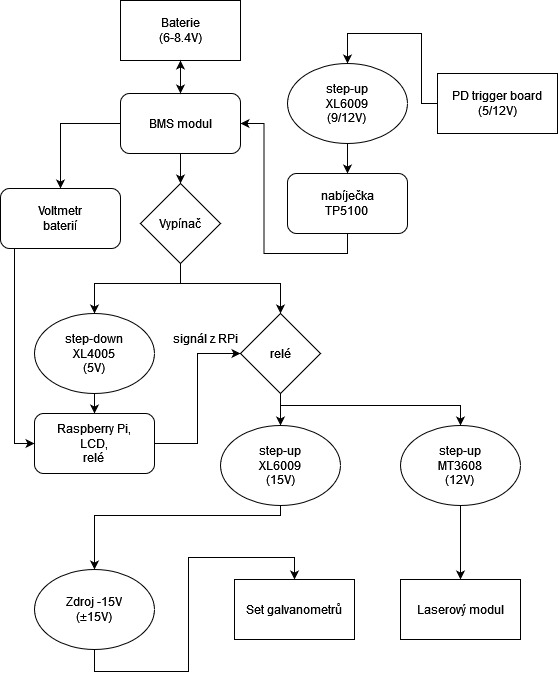
\includegraphics[width=\textwidth]{img/power-schem-full.jpg}
  \caption{\label{fig:power-schem-full} Celkové schéma napájení komponentů projektoru}
\end{figure}

\subsection{Akumulátory}
K napájení projektoru byly využity 4 Lithium-iontové akumulátory Samsung INR~18650 s~kapacitou 3~450~mAh~a jmenovitým napětím 3,7~V. Ty~byly zapojeny nejdříve po~dvojicích paralelně a~následně byly tyto dvojice zapojeny sériově. Konečný článek tedy dosahuje jmenovitého napětí 7,4~V.
\
\subsection{BMS modul}
Na baterie byl~napojen ochranný BMS~(Battery management system) modul, který ji~chrání před následujícími stavy:
\begin{itemize}
  \item odběr vysokého proudu (zkrat),
  \item přebití,
  \item vybití,
  \item nevybalancované články.
\end{itemize}
Modul články balancuje a~v případě, že nastane jiný z~nežádoucích stavů, ji~odpojí. Modul je~na~obrázku~\ref{fig:BMS}.


\begin{figure}[htb]
  \centering
  \begin{minipage}{0.45\textwidth}
    \centering
  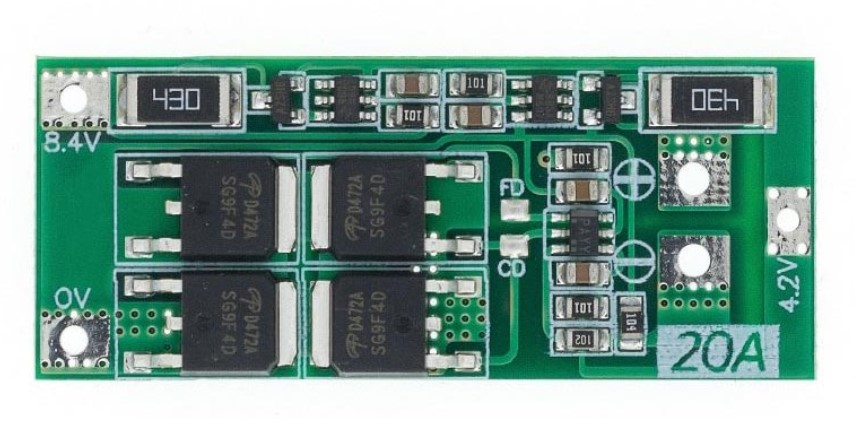
\includegraphics[width=0.8\textwidth]{img/BMS.jpg}
  \caption{\label{fig:BMS} BMS~Modul se~třemi kontakty pro~sérii baterií (0~V, 4,2~V a~8,4~V) a~výstupními kontakty ($(+)$ a~$(-)$)~\cite{laskakit-BMS}}
  \end{minipage}\hfill
  \begin{minipage}{0.45\textwidth}
    \centering
  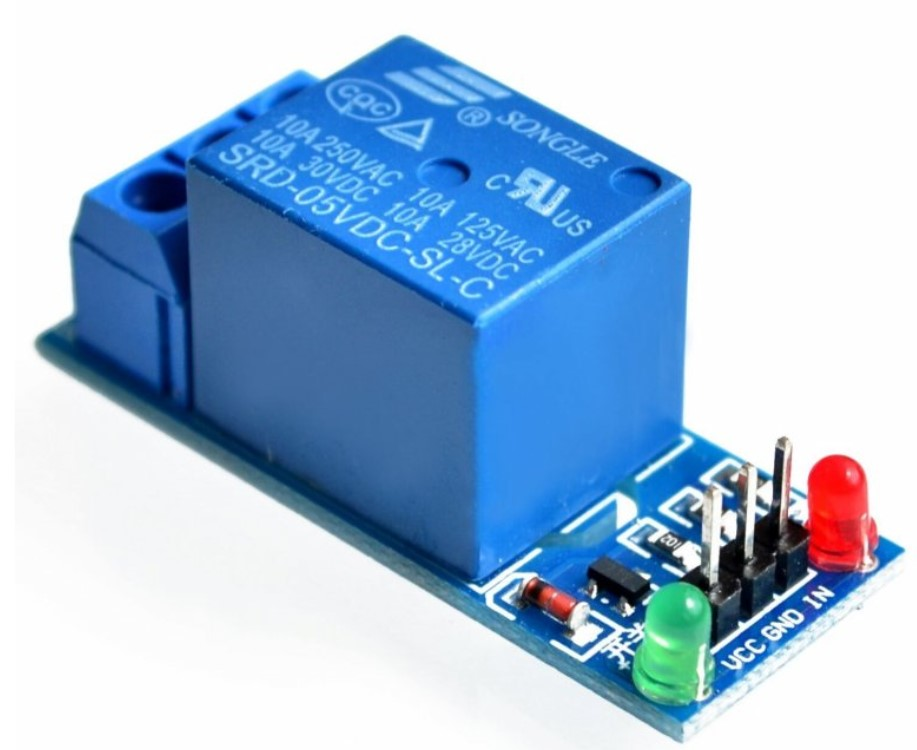
\includegraphics[width=0.8\textwidth]{img/relay.jpg}
  \caption{\label{fig:relay} Relé modul~\cite{laskakit-relay}}
  \end{minipage}
\end{figure}

\subsection{Relé modul}
V projektoru byl~využit relé modul pro~připojování komponentů s~vysokým odběrem pouze ve~chvílích, kdy~jsou využívány. Jedná se~o~set galvanometrů, laserový modul a~větrák, ty~jsou připojeny jen~ve~chvílích, kdy~projektor promítá.

Relé modul je~ovládán jedním kontaktem spojeným s~Raspberry Pi~a~je~umístěn mezi bateriemi a~měniči napětí, proto stačí pouze jeden na~více napěťových větví. Je~vidět na~obrazku~\ref{fig:relay}

\subsection{Nabíjecí obvod}
Zapojený nabíjecí obvod je~vidět na~obrázku~\ref{fig:hw_charging_circuit}.

\begin{figure}[htb]
  \centering
  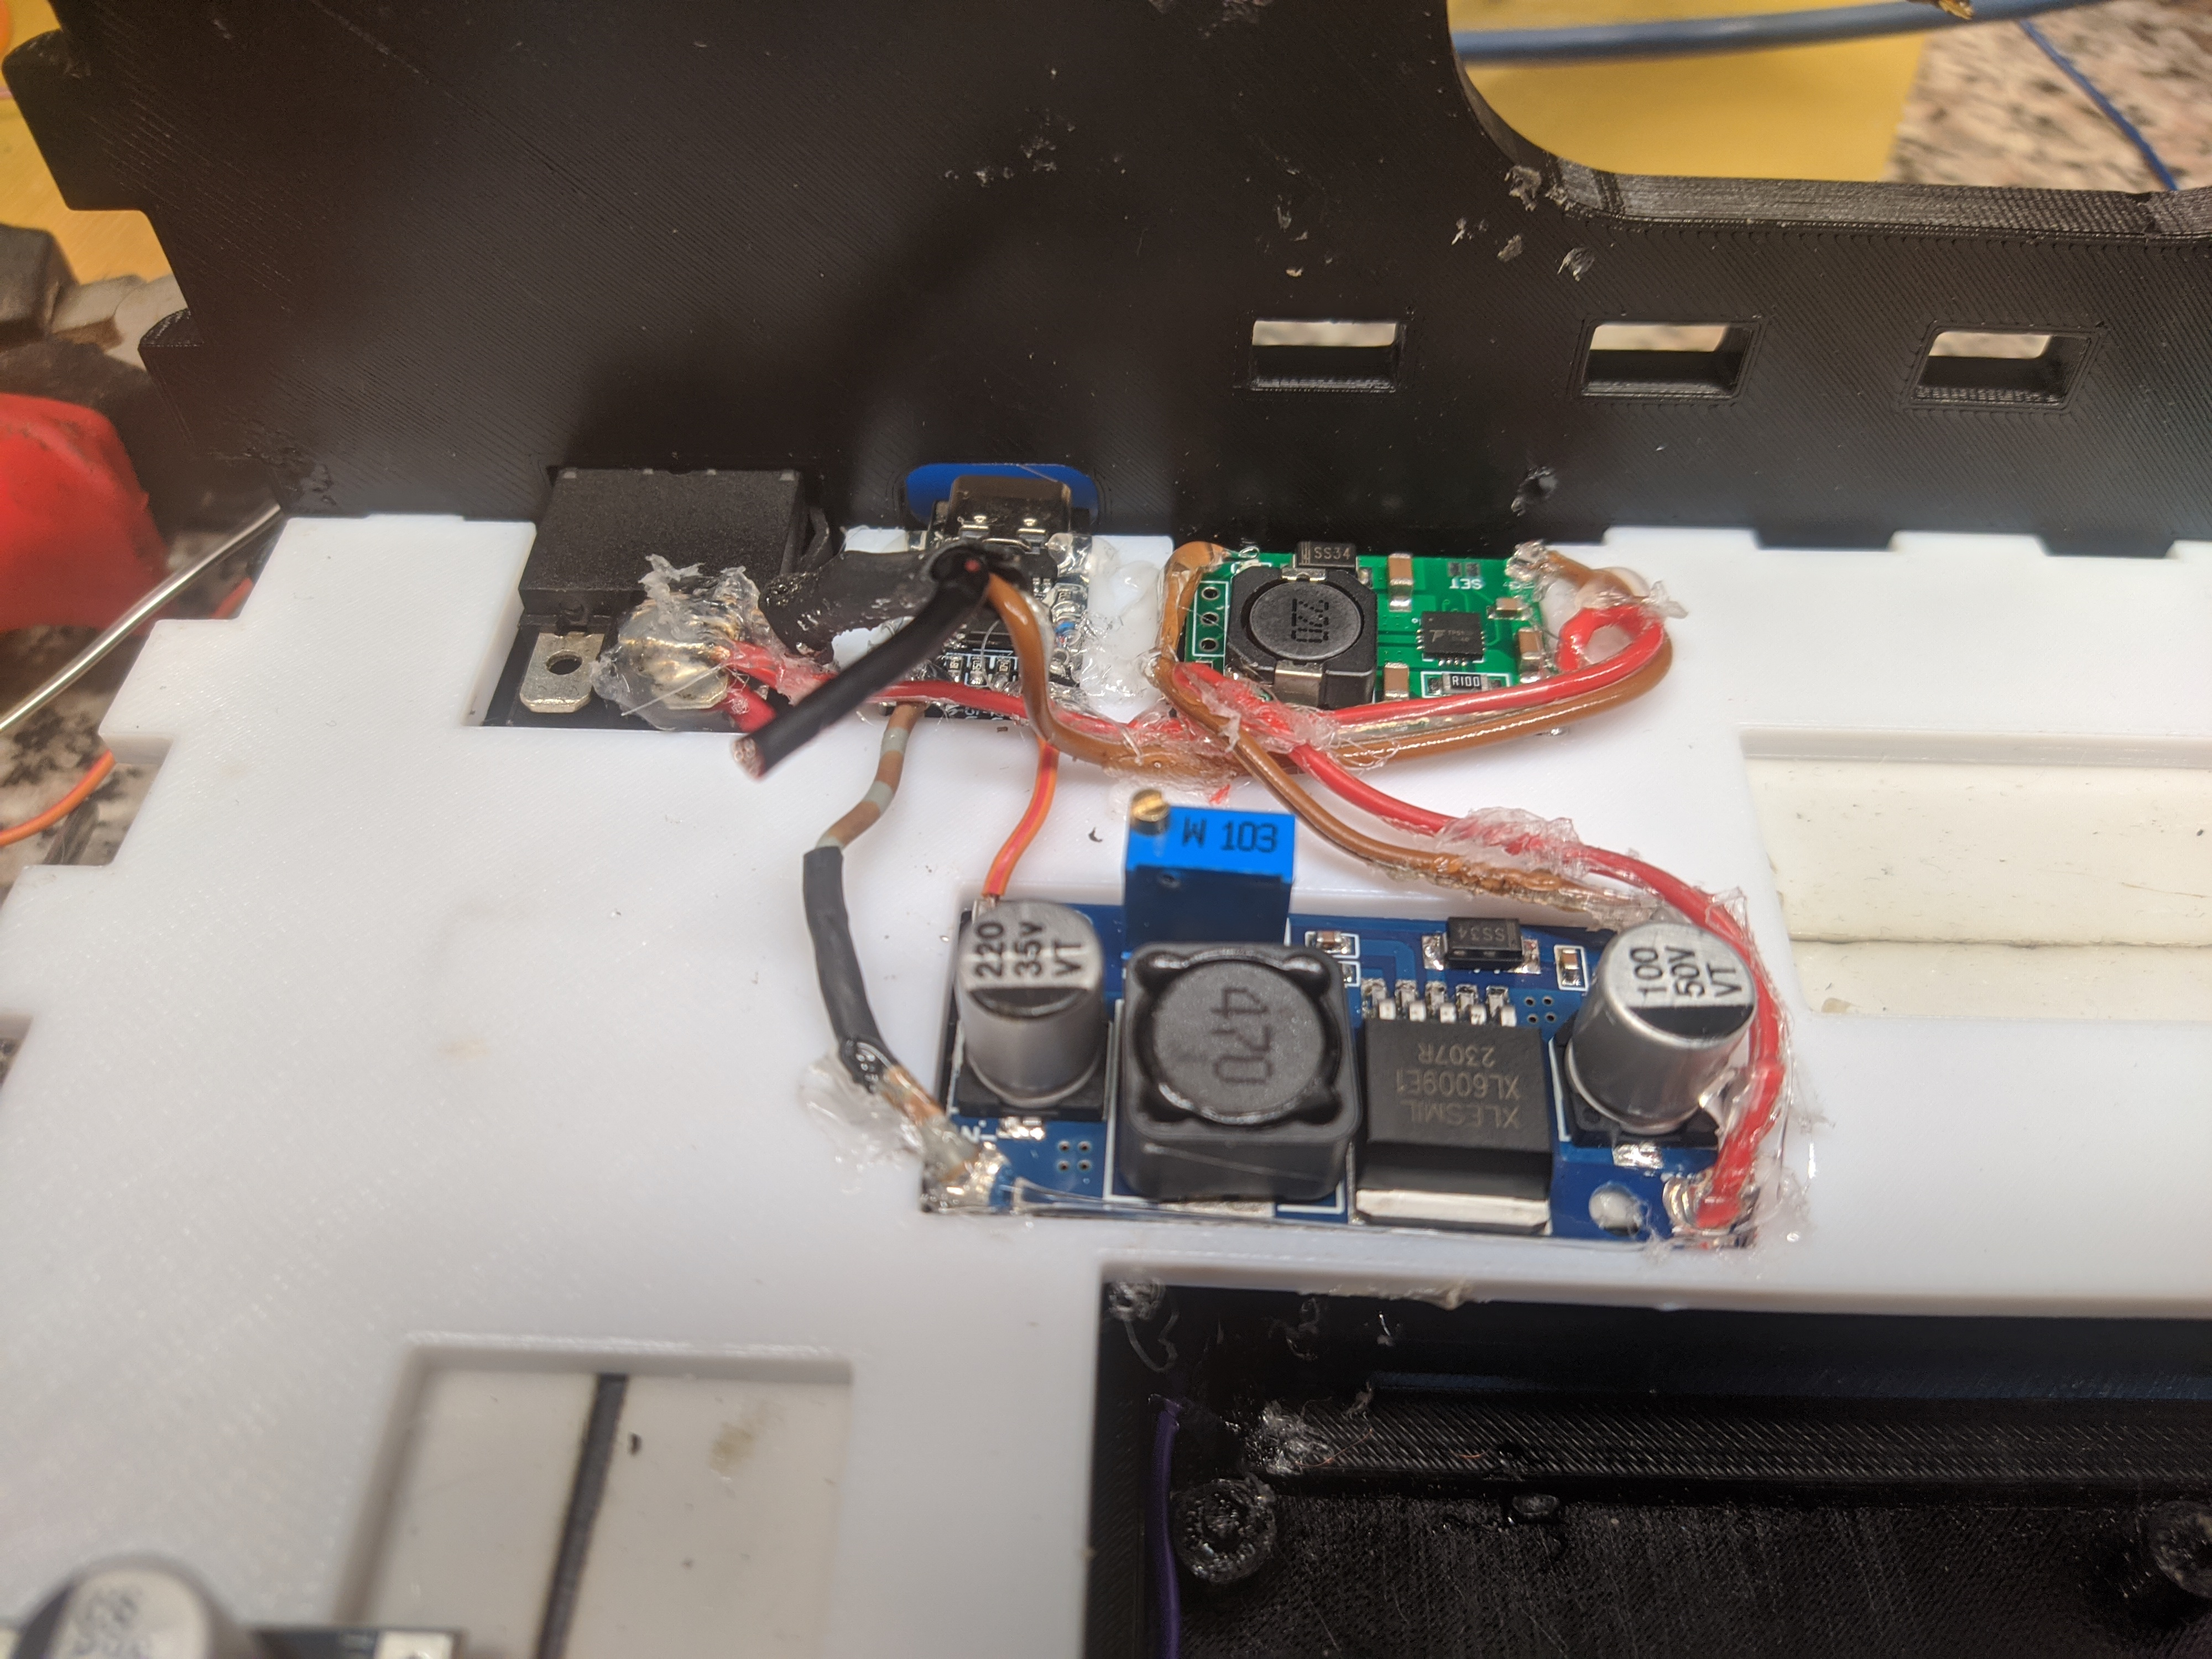
\includegraphics[width=0.8\textwidth]{img/hw_charging_circuit.jpg}
  \caption{\label{fig:hw_charging_circuit} Zapojený nabíjecí obvod}
\end{figure}

\subsubsection{Power Delivery (PD) trigger deska}
K nabíjení baterie je~využíván USB-C port podporující moderní protokoly rychlého nabíjení (hlavně Power Delivery a~Quick Charge).
Ten se~nachází na~desce s~integrovaným obvodem, který přes port komunikuje s~adaptérem v~zásuvce, pokud adaptér podporuje rychlé nabíjení, čip od~něj vyžádá napětí 12~V, které deska převádí na~výstupní kontakty viditelné na~obrázku~\ref{fig:PDtrig}. Protože deska \uv{vyvolá} dané napětí, označuje se~PD~trigger board (deska).

\begin{figure}[htb]
  \centering
  \begin{minipage}{0.25\textwidth}
    \centering
  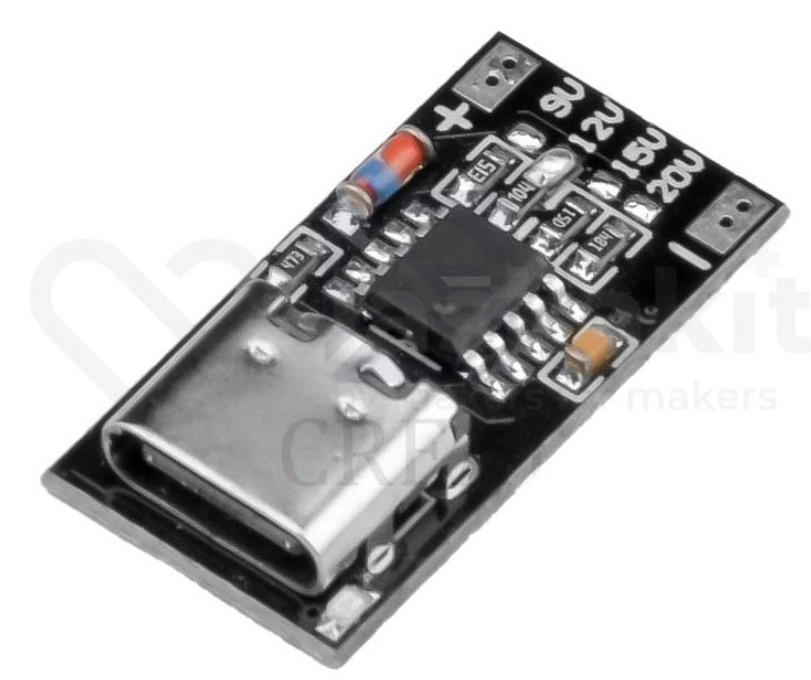
\includegraphics[width=1\textwidth]{img/PDtrig.jpg}
  \caption{\label{fig:PDtrig} Power Delivery trigger board~\cite{laskakit-PD}}
  \end{minipage}\hfill
  \begin{minipage}{0.35\textwidth}
    \centering
  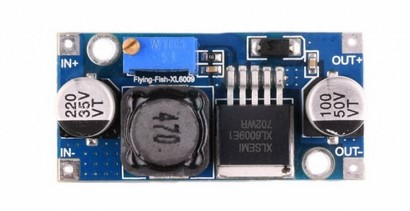
\includegraphics[width=1\textwidth]{img/XL6009.jpg}
  \caption{\label{fig:XL6009} Step-up měnič s~čipem XL6009~\cite{laskakit-XL6009}}
  \end{minipage}\hfill
  \begin{minipage}{0.3\textwidth}
    \centering
    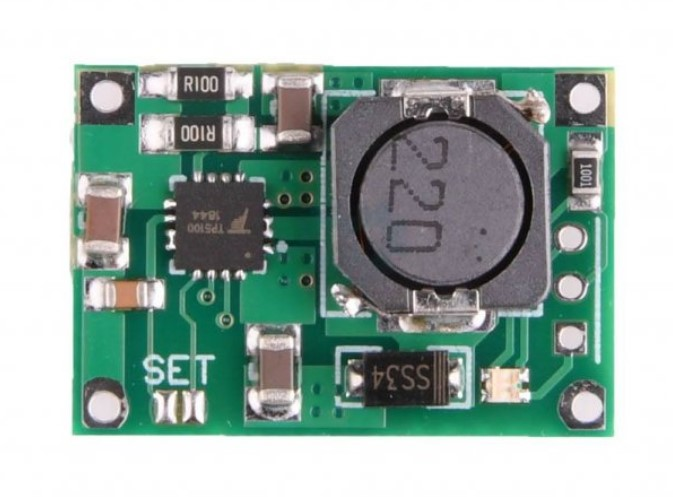
\includegraphics[width=0.8\textwidth]{img/TP5100.jpg}
    \caption{\label{fig:TP5100} Modul nabíječky dvou sériově zapojených Li-ion baterií~\cite{laskakit-TP5100}}
  \end{minipage}
\end{figure}

\subsubsection{Step up~měnič s~čipem XL6009}
Pokud ovšem připojený adaptér nepodporuje žádný rychlonabíjecí protokol, na~výstupech desky bude napětí pouze 5~V, na~kterém standartně běží USB~připojení. Proto je~k~PD~trigger board připojen step-up měnič nastavený na~9~V.
Pokud z~PD~desky bude vycházet napětí 5~V, step-up jej~zvýší na~9~V. Pokud z~PD~desky bude vycházet 12~V, napětí step-up projde beze změny.

\subsubsection{TP5100}
K ovládání průběhu nabíjení byl~využit modul pro~nabíjení Li-ionových baterií s~čipem TP5100. Ten~zajišťuje konstantní proud a~napětí, které posílá na~kontakty BMS~obvodu. Další z~jeho funkcí je~automatické ukončení nabíjení ve~chvíli, kdy~baterie dosáhnou napětí 8,4~V. Je~to~jedinečný modul, který umožňuje nabíjení dvoučlánkových lithium-iontových akumulátorů.

\subsection{Vypínač}
K bateriím je~neustále připojený jen~BMS modul a~nabíjecí obvod, všechny ostatní obvody jsou přemostěny vypínačem. Je~tedy možné baterie nabíjet, i~když jsou všechny ostatní obvody odpojené. Vypínač je~vidět na~obrázku~\ref{fig:hw_charging_circuit}.

\subsection{Napěťové větve}
Různé komponenty projektoru pracují s~různými napětími. Je~tedy potřeba napětí baterií převést na~několik napěťových větví. Jedná se~o~větve:

\begin{itemize}
  \item 5V --- Napětí Raspberry Pi, LCD~a relé modulu; Zajištěno step-down měničem s~čipem XL4005 (viz obrázek~\ref{fig:XL4005}.)
  \item 12V --- Napětí Laserového modulu; Zajištěno step-up měničem s~čipem MT3608 (viz obrázek~\ref{fig:MT3608}.)
  \item Symetrické napětí $\pm{}15$~V~--- Napětí řídící desky galvanmetrů; Kladná větev je~zajištěna step-up měničem s~čipem XL6009 (viz obrázek~\ref{fig:XL6009}.), záporná větev je~zajištěna obvodem zdroje $-15$~V~na~HAT~DPS (viz kapitola~\ref{sec:negative-ps}).
\end{itemize}


\begin{figure}[htb]
  \centering
  \begin{minipage}{0.45\textwidth}
    \centering
  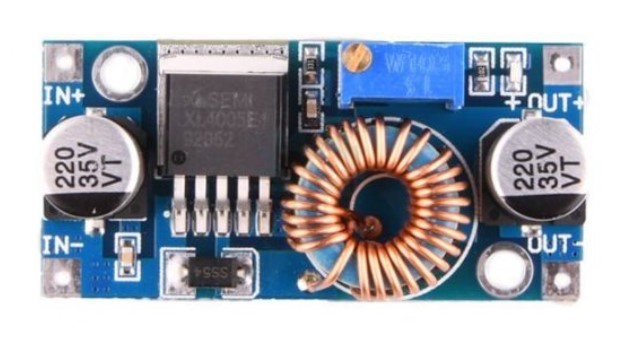
\includegraphics[width=0.8\textwidth]{img/XL4005.jpg}
  \caption{\label{fig:XL4005} Step-down měnič s~čipem XL4005~\cite{laskakit-XL4005}}
  \end{minipage}\hfill
  \begin{minipage}{0.45\textwidth}
    \centering
  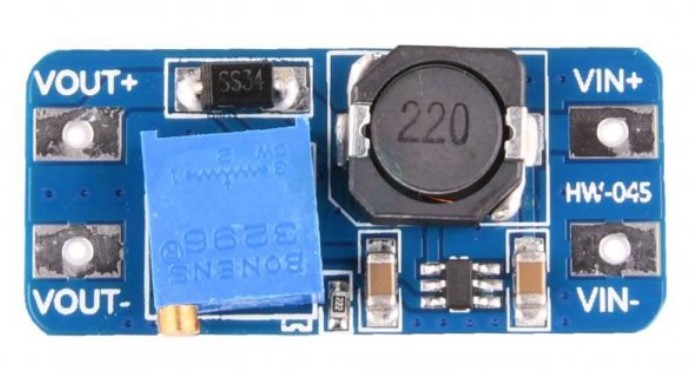
\includegraphics[width=0.8\textwidth]{img/MT3608.jpg}
  \caption{\label{fig:MT3608} Step-up měnič s~čipem MT3608~\cite{laskakit-MT3608}}
  \end{minipage}
\end{figure}
